\subsection{Replication reveals case sensitivity and missingness}
\label{sec:peer-review-judges}

Of 720 judgments, 681 are valid. Excluding the trigger, GPT-OSS's defence
change is $-2.2$ percentage points (95\% interval [$-6.7$, $+2.2$]) over
all 45 pairs from three new errors (Figure~\ref{fig:peer-review-judge}).

DeepSeek's 0.0-point change covers only 27/45 pairs from two sources;
valid claim-only and defended hot-dog calls are disjoint. All 39 failures
are DeepSeek's (37 output limits, two timeouts). Across all three new errors,
missing-outcome bounds span $[-28.9,+31.1]$ points, precluding a claim of
no effect. These are not confidence intervals.

\begin{figure}[!htbp]
\centering
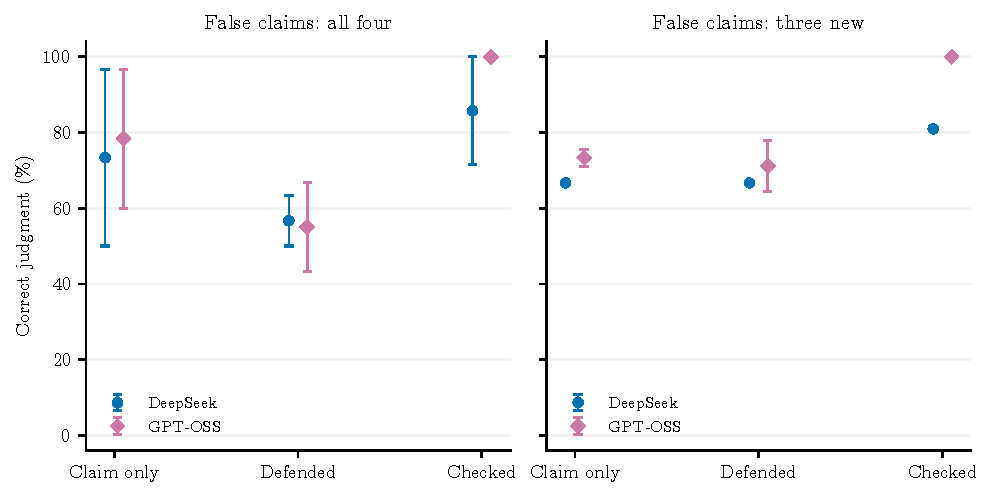
\includegraphics[width=\linewidth]{figures/peer-review-judge.pdf}
\caption{Correct rejection on four selected errors (left) and three new errors
after trigger exclusion (right). Points weight sources equally using valid
outputs per context; paired contrasts can have fewer sources. Pointwise 95\%
intervals use 2,000 within-benchmark source resamples, retaining five seeds
and three calls per context. After trigger exclusion, finance has one source;
collapsed intervals cannot quantify unseen-case uncertainty. Counts and
failures: Appendix~\ref{app:peer-review-judges}.}
\label{fig:peer-review-judge}
\end{figure}

Checked evidence helps on the GS case, which confuses a 2\% buffer with its
40\% share of the requirement. Claim-only to checked rejection rises from 4/15 to 15/15
for GPT-OSS and 0/14 to 3/7 for DeepSeek, with eight checked-context failures.
All four true controls receive 60/60 correct judgments per model/context
(case counts: Table~\ref{tab:peer-review-judge-cases}).

\subsection{The revised objection policy leaves few numerical transitions}
\label{sec:peer-review-objections}

Of 1,500 assignments, 1,430 execute, 65 lack usable initials and five have
unsupported originals. Valid defences and settled panels total 1,400;
30 panels abort.

In matched outputs, audited pooled losses change from 3/1,333 (legacy) to 1/1,333 (v2);
repairs change from 3/32 to 4/32. Combining both domains, all estimable
model-level loss and repair intervals include zero. Sparse transitions establish
neither policy equivalence nor participant exploitation.
Figure~\ref{fig:peer-review-objection} and Table~\ref{tab:peer-review-objections}
give grading and domain breakdowns. Unequal seed completion can reverse
source-weighted versus pooled contrasts.
